\subsection{赤外線をつかった家電}

\begin{figure}[H]
  \begin{minipage}[t]{0.3\columnwidth}
    \centering
 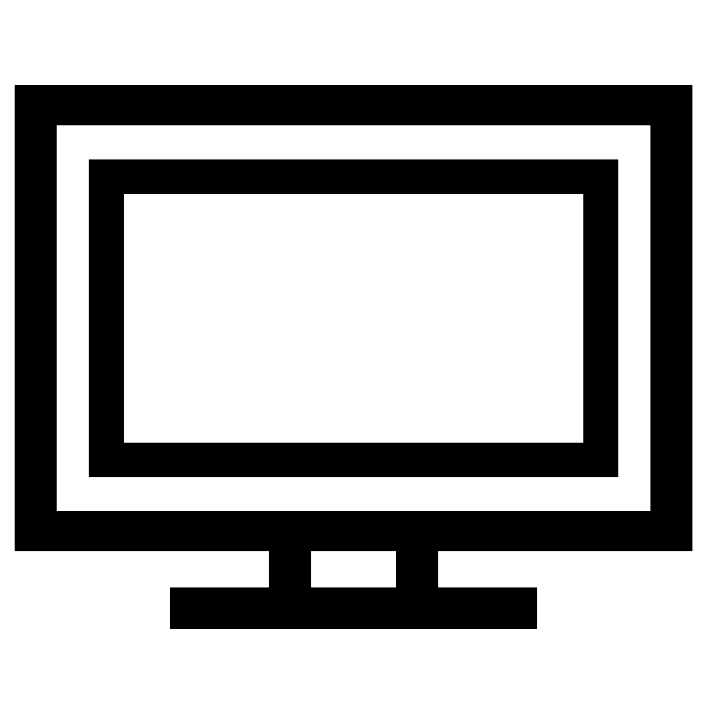
\includegraphics[scale=0.1]{images/chap05/text05-img038.png}
    \caption{テレビ}
  \end{minipage}
  %\hspace{0.01\columnwidth} % ここで隙間作成
  \begin{minipage}[t]{0.3\columnwidth}
    \centering
    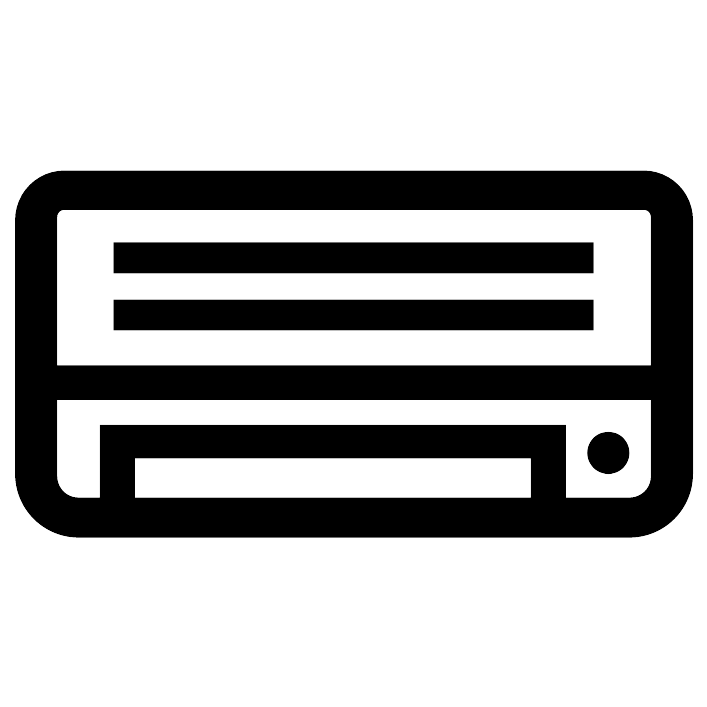
\includegraphics[scale=0.1]{images/chap05/text05-img039.png}
    \caption{エアコン}
  \end{minipage}
  \begin{minipage}[t]{0.3\columnwidth}
    \centering
    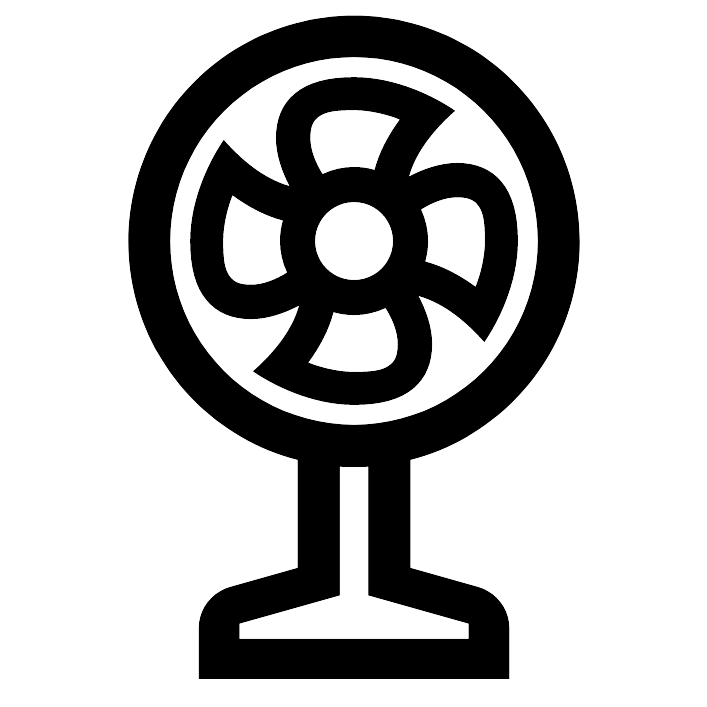
\includegraphics[scale=0.1]{images/chap05/text05-img040.png}
    \caption{せんぷう機}
  \end{minipage}
\end{figure}

テレビ、エアコン、せんぷう機などはリモコンを使って動作を制御しています。ボタンを押せば電源が点いたり、風量や音量を調節できます。これは赤外線を使って家電を制御しています。電源を入れるときはリモコンから電源を入れるための赤外線信号が送られます。家電はそれを受け取り、信号で決められた動作をします。